\documentclass[10pt,a4paper,twocolumn]{article}
\newcommand{\runningtitle}{Baryon-antibaryon population reconstruction}
\newcommand{\paperfooter}{Research manuscript | 8 October 2026}
\usepackage[utf8]{inputenc}
\usepackage[T1]{fontenc}
\usepackage{lmodern}
\usepackage[margin=17mm,top=18mm,bottom=19mm,columnsep=6.5mm]{geometry}
\usepackage{amsmath,amssymb,array,booktabs,graphicx,xcolor,microtype}
\usepackage[authoryear,round]{natbib}
\usepackage{caption,stfloats,fancyhdr,balance}
\usepackage{multicol}
\usepackage[unicode,colorlinks=true,linkcolor=navy,citecolor=navy,urlcolor=navy]{hyperref}
\definecolor{navy}{HTML}{173B56}
\setlength{\parindent}{1em}
\setlength{\parskip}{1pt}
\setlength{\emergencystretch}{1.7em}
\setlength{\intextsep}{9pt}
\setlength{\textfloatsep}{11pt}
\setlength{\dbltextfloatsep}{11pt}
\setcounter{topnumber}{3}
\setcounter{dbltopnumber}{2}
\renewcommand{\topfraction}{.92}
\renewcommand{\dbltopfraction}{.95}
\renewcommand{\textfraction}{.08}
\renewcommand{\floatpagefraction}{.82}
\renewcommand{\dblfloatpagefraction}{.82}
\captionsetup{font=small,labelfont=bf,labelsep=period,skip=5pt}
\pagestyle{fancy}
\fancyhf{}
\fancyhead[L]{\footnotesize\color{navy}\runningtitle}
\fancyhead[R]{\footnotesize Andrés Germán García}
\fancyfoot[L]{\footnotesize\paperfooter}
\fancyfoot[R]{\footnotesize\thepage}
\setlength{\headheight}{13pt}
\renewcommand{\headrulewidth}{.35pt}
\newcommand{\fB}{f^{(s)}_{B\bar B}}
\newcommand{\sB}{s_{B+\bar B}}
\newcommand{\stot}{s_{\mathrm{tot}}}
\newcommand{\shad}{s_{\mathrm{had}}}
\newcommand{\sL}{s_{\mathrm{light}}}
\newcommand{\YB}{Y_{\Delta B}}
\newcommand{\doi}[1]{\href{https://doi.org/#1}{doi:#1}}
\newcommand{\fulltitle}[3]{%
\twocolumn[%
\begin{center}
{\fontsize{18}{20.5}\selectfont\bfseries\color{navy}#1\par}
\vspace{8pt}
{\normalsize Andrés Germán García\par}
{\small #2\par}
\vspace{7pt}
{\small #3\par}
\end{center}
\vspace{6pt}
\begin{minipage}{\textwidth}
\textbf{\abstractlabel.} \abstracttext
\vspace{6pt}\par
\textbf{\keywordslabel:} \keywordstext
\end{minipage}
\vspace{15pt}
]%
}


\newcommand{\abstractlabel}{Abstract}
\newcommand{\keywordslabel}{Keywords}
\newcommand{\abstracttext}{The objective was to test whether known particle-species properties and current cosmological abundances can reconstruct baryon and antibaryon populations during the annihilation epoch, and to compare these quantities with published knowledge. Rest masses from HRG inventories based on PDG2014, PDG2020, and PDG2025 were retained. Number densities were calculated using Bose-Einstein and Fermi-Dirac thermal distributions; baryon chemical potential was solved by imposing the observed excess per entropy unit at eight temperatures from 150 to 40 MeV. Bessel sums, independent integrals, and the rank of the net-abundance map were checked, and the published nucleon limit was compared. At 150 MeV, PDG2025 yielded approximately $1.7222\times10^{37}$ baryons and the same rounded antibaryon density per cm$^3$, with difference $4.0110\times10^{29}$ cm$^{-3}$. At 40 MeV, $1.9166\times10^{28}$ and $1.4894\times10^{28}$ cm$^{-3}$ were distinguished, respectively. Total yield decreased by 7.0323 orders of magnitude. Baryons other than protons and neutrons supplied 74.42\% at 150 MeV and 1.525\% at 40 MeV in the symmetric control. Evaluation around the hadronic-transition reference of $156.5\pm1.5$ MeV quantified sensitivity to the starting temperature. The net map had rank one: present abundance alone did not select a unique initial pair population. Reconstruction was possible under stated temperature, equilibrium, and conservation assumptions. These quantities provide a reproducible reference for physical comparison. Cumulative reaction counts require integration of kinetic evolution.}
\newcommand{\keywordstext}{annihilation; baryon abundance; hadronic resonances; rest mass; retrospective reconstruction; thermal equilibrium.}
\hypersetup{pdftitle={Baryon-Antibaryon Population Reconstruction: Rest Masses and Cosmological Abundances},pdfauthor={Andrés Germán García}}
\begin{document}
\fulltitle{Baryon-Antibaryon Population Reconstruction:\\Rest Masses and Cosmological Abundances}{Independent Researcher, Mexico}{Thermal reconstruction and literature comparison | 8 October 2026}
\section{Introduction}
The present abundance of baryonic matter and known particle properties raise a retrospective question: can our rest masses, inventories, and calculations, together with current cosmological abundances, reconstruct how many baryons and antibaryons were present during the annihilation epoch, and how does that reconstruction compare with established knowledge? The cosmic microwave background and primordial nucleosynthesis constrain the small surviving net baryon excess \citep{Fields2025,Planck2020}. This excess and the total pair population are different quantities.

A hadron resonance gas (HRG) uses the rest masses, degeneracies, and charges of particle species to sum their populations and thermodynamic contributions \citep{Vovchenko2019}. These masses were already used in our calculations. Here, \emph{particle signatures} means these identifying catalog properties, rather than original spectral signals measured by this study. The model links such properties, a specified temperature, and equilibrium populations mathematically. Its usefulness at low temperature has been compared with lattice quantum chromodynamics, with agreement depending on the observable and proximity to the transition \citep{Bazavov2012}.

Annihilation removes equal numbers of baryons and antibaryons and preserves a pre-existing excess when baryon number is conserved. Inverse reactions also contribute to thermal evolution. \citet{Satarov2013} studied both contributions together with expansion and emphasized the importance of heavy antibaryon resonances above approximately 100 MeV. A useful comparison therefore separates equilibrium population reconstruction, the information supplied by current abundances, and the reaction history requiring kinetic calculation.

\textbf{The primary objective was to test whether particle-species properties and the present baryon abundance can reconstruct baryon and antibaryon numbers under annihilation-epoch conditions, and to compare that reconstruction with published results and approximations.} An inverse constraint linking the observed cosmic excess to the HRG baryon chemical potential was solved at eight temperatures. We also examined whether the present abundance alone uniquely determines an initial population. Complementary checks compared three public inventories, the literature's nucleon approximation, and a previous entropy reference \citep{Garcia2026}. The working hypothesis was that reconstruction requires an explicit temperature and thermal conditions in addition to masses and present abundance.

\section{Methods}
A mathematical retrospective reconstruction was performed using the rest masses and other properties already present in our HRG inventory. The current cosmological abundance was introduced as a constraint on early populations. Baryon, antibaryon, entropy, and net-excess densities were calculated separately; zero-chemical-potential entropy comparisons were retained as inventory checks.
\subsection{Design and input provenance}
The temperatures evaluated were
\[
T=150,\ 140,\ 120,\ 100,\ 80,\ 60,\ 50,\ 40\ {\rm MeV},
\]
The reconstruction solved for $\mu_B$ at each temperature with $\mu_Q=\mu_S=0$; the symmetric control also fixed $\mu_B=0$. Here $\mu_B$ controls the baryon-antibaryon imbalance, while $\mu_Q,\mu_S$ are the electric-charge and strangeness chemical potentials. Natural units, $\hbar=c=k_B=1$, were adopted, and all temperatures and masses were converted to GeV before summation. All species shared one temperature.

Only the \texttt{list.dat} files in the PDG2014, PDG2020, and PDG2025 directories of Thermal-FIST were used \citep{TFLists2026}. Inputs were frozen at revision \texttt{4086191e9522}; the supplement records the complete identifier, exact links, and SHA-256 hashes. The selected lists contain hadrons from the $u,d,s$ quark sector. Separate lists of hadrons containing a charm quark, nuclei, and other sectors were not added and do not represent every particle in the PDG.

Table~\ref{tab:inventory} records the effective input sizes. Commented lines and zero-degeneracy contributions were discarded. File masses and degeneracies were retained, including spin assignments adopted by the list maintainers.

\begin{table}[t]
\centering\small
\caption{Inventory of the lists used. The last two columns include antiparticles and only positive-degeneracy entries.}
\label{tab:inventory}
\setlength{\tabcolsep}{3.6pt}
\begin{tabular}{lrrr}\toprule
List & Rows & Active species & $B+\bar B$\\\midrule
PDG2014 & 219 & 387 & 260\\
PDG2020 & 242 & 433 & 298\\
PDG2025 & 248 & 443 & 292\\
\bottomrule\end{tabular}
\end{table}

Reduced values were transcribed from \citet{Garcia2026} and stored as a separate input with four significant digits. No ad hoc reduced list was constructed to force that table. The PDG-column values reported below are results of this study calculated from published particle data; these same percentages were not extracted from an external publication.

\subsection{Observable and thermodynamic accounting}
The instantaneous fraction was defined as
\begin{equation}
\fB(T)=\frac{\sB(T)}{\stot(T)},
\label{eq:f}
\end{equation}
where $\sB$ includes all active baryons and antibaryons in the selected list. At vanishing chemical potentials this sector is symmetric. Hadronic entropy was written as
\begin{equation}
\shad=\sB+s_{\rm mes},
\end{equation}
and the entropy of the plasma considered as
\begin{equation}
\stot=\shad+s_\gamma+s_{e^\pm}+s_{\mu^\pm}+s_{\nu\bar\nu}.
\label{eq:den}
\end{equation}
To assess the denominator effect, we also calculated
\begin{equation}
f_{\rm had}(T)=\frac{\sB(T)}{\shad(T)}.
\label{eq:fhad}
\end{equation}
Neither fraction is a net abundance, an annihilation rate, or a share of present-day photons with identifiable ancestry.

\subsection{Entropy per particle species and antiparticle counting}
For each massive species in an equilibrium ideal gas, at $\mu_i=0$, we evaluated
\begin{align}
s_i(T)&=\frac{g_i m_i^2T}{2\pi^2}
\sum_{k=1}^{K_{\max}}c_{i,k}\,A_{i,k},\label{eq:entropy}\\
A_{i,k}&=\frac{4}{k^2}K_2(kx_i)+\frac{x_i}{k}K_1(kx_i),\\
x_i&=\frac{m_i}{T}.\nonumber
\end{align}
$K_1$ and $K_2$ are modified Bessel functions of the second kind; $g_i$ denotes spin degeneracy. We used $c_{i,k}=1$ for bosons and $c_{i,k}=(-1)^{k+1}$ for fermions. These coefficients implement Bose-Einstein distributions for bosons and Fermi-Dirac distributions for fermions, describing occupation of energy states at the chosen temperature. Keeping only $k=1$ recovers the Maxwell-Boltzmann approximation. These physical population distributions differ from statistical tests of measurements.

Each file contains one member of particle-antiparticle pairs. Its contribution was multiplied by two if at least one of its $B,Q,S,C$ quantum numbers was nonzero, and by one for self-conjugate states. Charge and isospin states already appear as individual entries, so no extra isospin degeneracy was introduced. The implementation checked that there were no negative PDG identifiers or duplicate entries before applying this rule.

Nominal masses and zero resonance widths were used. Decay tables were neither propagated nor added again to the denominator: the observable was the entropy of the equilibrium inventory rather than final decay yields. Excluded-volume effects, attractive or repulsive interactions, and fits to lattice data were not included.

\subsection{Reconstruction of particle numbers}
A particle species meant one type identified by an inventory entry, with spin states counted by $g_i$. Number density was evaluated in addition to entropy using the ideal-gas thermal distributions \citep{Vovchenko2019}:
\begin{equation}
n_i^{\rm eq}(T)=\frac{g_i m_i^2T}{2\pi^2}
\sum_{k=1}^{96}\frac{c_{i,k}}{k}K_2(km_i/T).
\label{eq:number}
\end{equation}
Here $g_i$ belonged to one particle species; its antiparticle was recorded separately at the same density for $\mu_i=0$. All active baryonic entries were checked to have $|B_i|=1$. Summing over $B_i=+1$ and $B_i=-1$ gave $n_B$ and $n_{\bar B}$, respectively. We defined
\begin{align}
n_\Sigma&=n_B+n_{\bar B}, & \Delta n_B&=n_B-n_{\bar B},\\
Y_\Sigma&=n_\Sigma/\stot, & \YB&=\Delta n_B/\stot.
\label{eq:yields}
\end{align}
The $\mu_B=0$ control gave $\Delta n_B=0$; the finite-excess reconstruction is described below. Potential pair bookkeeping used $n_{\rm pair}=\min(n_B,n_{\bar B})$, rather than counting bound pairs or reaction events.

Natural-unit densities were divided by $(\hbar c)^3$ to obtain ${\rm cm^{-3}}$, with $\hbar c=1.973269804\times10^{-14}$ GeV cm \citep{Robinson2025}. Mean particle number in a specified volume is $N_i=n_iV$. Densities were exported for each particle species and temperature. Reconstruction inferred these equilibrium populations from their properties and the cosmological constraint; physical regeneration would require integrating inverse-production and annihilation rates. The initial point $T_i=150$ MeV was the upper end of the computational grid, without assigning it a cosmic age or identifying it with a kinetic annihilation onset.

\subsection{Common light sector}
Photons were treated as massless bosons with $g=2$; electrons and positrons as massless fermions with combined $g=4$; and three neutrino flavors plus antineutrinos as massless fermions with six combined helicity states. For each relativistic component,
\begin{equation}
s_{\rm rel}=\frac{2\pi^2}{45}gT^3
\begin{cases}
1,&\text{bosons},\\
7/8,&\text{fermions}.
\end{cases}
\end{equation}
Muons and antimuons were evaluated with Eq.~\eqref{eq:entropy}, combined $g=4$, and $m_\mu=0.1056583755$ GeV \citep{PDG2025}. This same light sector was used for all three lists. The massless-electron approximation was separately checked by integration with the physical electron mass.

\subsection{Normalization to the relic and cosmological abundances}
External inputs were $\eta=(6.12\pm0.04)\times10^{-10}$ and $\YB^{\rm ref}=\eta/7.04$ \citep{Fields2025}. The factor 7.04 was the standard entropy-per-photon approximation after $e^+e^-$ annihilation. Yields were used to compare epochs with different dilution, instead of comparing physical densities directly. We calculated
\begin{equation}
\mathcal Q(T)=\frac{Y_\Sigma^{\rm eq}(T)}{\YB^{\rm ref}}.
\label{eq:populationratio}
\end{equation}
$\mathcal Q$ is the total thermal number per reference net baryon, and $\mathcal Q/2$ is its symmetric pair bookkeeping. It is not a measured survival fraction.

We used $T_{\gamma0}=2.7255\pm0.0006$ K, rounded from \citet{Fixsen2009}, to connect this normalization with the present:
\begin{align}
n_{\gamma0}&=\frac{2\zeta(3)}{\pi^2}
\left(\frac{k_BT_{\gamma0}}{\hbar c}\right)^3,\\
s_0/k_B&\simeq7.04\,n_{\gamma0}, & n_{b0}&=\eta n_{\gamma0}.
\label{eq:today}
\end{align}
$n_{b0}$ counts baryon-number units (nucleons), including those in nuclei, rather than atoms. An adiabatic comparison obeys $s(T)V(T)=s_0V_0$, hence $N_\Sigma^{\rm eq}=Y_\Sigma^{\rm eq}s_0V_0$ and $N_{\Delta B}^{\rm ref}=\YB^{\rm ref}s_0V_0$. This supplied a common comoving normalization conditional on entropy and net-baryon conservation.

Using the primordial baryon fraction in $^4$He, $Y_p=0.245\pm0.003$, and $(D/H)_{\rm P}=(2.508\pm0.029)\times10^{-5}$ \citep{Fields2025}, we calculated a primordial-composition equivalent at today's mean cosmic density:
\begin{align}
n_{{\rm H},0}^{\rm prim}&\simeq(1-Y_p)n_{b0},\\
n_{{}^4{\rm He},0}^{\rm prim}&\simeq Y_p n_{b0}/4,\\
n_{{\rm D},0}^{\rm prim}&\simeq(D/H)_{\rm P}n_{{\rm H},0}^{\rm prim}.
\label{eq:hydrogen}
\end{align}
Small nuclear-binding and trace-nuclide corrections were neglected. Stellar processing and ionization were not modeled, so these conversions do not constitute a present neutral-hydrogen measurement. First-order uncertainties in $\eta,T_{\gamma0},Y_p,D/H$ were propagated assuming independent inputs: $\sigma_F^2\simeq\sum_j(\partial F/\partial x_j)^2\sigma_{x_j}^2$. Outputs share inputs and have correlated errors. These uncertainties were not assigned to the HRG model.

\subsection{Inverse inference from the current abundance}
The central constraint was conservation of net yield under adiabatic expansion and without baryon-number violation:
\begin{equation}
\frac{\Delta n_B(T,\alpha)}{\stot(T,\alpha)}
=\frac{\eta}{7.04},\qquad \alpha=\mu_B/T.
\label{eq:inverse}
\end{equation}
The central value of $\eta$ was used for each list and temperature. Its observational uncertainty was not propagated to inverse populations; these are estimates conditional on central inputs.

For entries with $B_i=+1$, we defined $a_{i,k}=g_i m_i^2T c_{i,k}K_2(kx_i)/(2\pi^2 k)$ and $b_{i,k}=g_i m_i^2T c_{i,k}A_{i,k}/(2\pi^2)$. Antiparticles had the opposite potential. We evaluated
\begin{align}
n_\Sigma(T,\alpha)&=2\sum_{i,k}a_{i,k}\cosh(k\alpha),\\
\Delta n_B(T,\alpha)&=2\sum_{i,k}a_{i,k}\sinh(k\alpha),\\
\sB(T,\alpha)&=2\sum_{i,k}\bigl[b_{i,k}\cosh(k\alpha)\nonumber\\
&\hspace{18mm}-\alpha a_{i,k}\sinh(k\alpha)\bigr].
\label{eq:inversekernels}
\end{align}
This avoided subtracting nearly equal densities to recover the small excess. Mesonic and light entropy were added, and Eq.~\eqref{eq:inverse} was solved by Brent's method on $0\leq\alpha\leq1$, with absolute tolerance $10^{-18}$ and relative tolerance $10^{-13}$. Populations were recovered as $n_B=(n_\Sigma+\Delta n_B)/2$ and $n_{\bar B}=(n_\Sigma-\Delta n_B)/2$.

Masses, spin, and charges came from the catalog; $\eta$ and today's CMB temperature were observational inputs. Early temperature was specified, and the ideal HRG supplied the thermal relation needed to infer the total. Masses were not fitted, and no new spectral signatures were analyzed. Fixing $\mu_Q=\mu_S=0$ did not simultaneously impose electric neutrality and zero net strangeness; this scope was retained in interpretation.

\subsection{Initial temperature and physical reference}
The main grid retained $T_i=150$ MeV to preserve comparison with our earlier calculations. Its scale was assessed using the lattice-QCD transition estimate of \citet{Bazavov2019}, $T_c=156.5\pm1.5$ MeV at zero chemical potentials. This reference characterizes the emergence of hadrons, without fixing a universal annihilation onset. Inverse solutions were repeated at 150, 155, 156.5, and 158 MeV for all three lists and at 96 and 192 terms. Kelvin conversion used $T_{\rm K}=10^6T_{\rm MeV}/k_B$, with $k_B=8.617333262\times10^{-5}$ eV K$^{-1}$ \citep{Robinson2025}. Near-$T_c$ evaluation was treated as ideal-HRG sensitivity; the published $T_c$ uncertainty was not interpreted as a complete physical uncertainty on our densities.

\subsection{Uniqueness test and literature comparison}
The information in net abundance was examined through the linear yield map
\begin{equation}
Y_{\Delta B}=\begin{pmatrix}1&-1\end{pmatrix}
\begin{pmatrix}Y_B\\Y_{\bar B}\end{pmatrix}.
\label{eq:rank}
\end{equation}
Its rank and null direction were evaluated. Adding a quantity $q$ to both components preserves their difference. Four algebraic examples had totals of 0.1, 1, 10, and 100 times the reconstructed total at 150 MeV, with the same excess. They examined uniqueness under conservation; they did not establish kinetic histories or physically realizable equilibrium states at a common temperature.

We also evaluated the Maxwell-Boltzmann nucleon limit underlying Eq. (19) of \citet{Satarov2013}, using our list's distinct proton and neutron masses:
\begin{equation}
n_N^{\rm MB}(T)=\sum_{i=p,n}
\frac{g_i m_i^2T}{2\pi^2}K_2(m_i/T).
\label{eq:nucleonMB}
\end{equation}
It was compared with the Fermi-Dirac proton-plus-neutron density and with all HRG baryons at $\mu_B=0$. Nucleon share and relative distribution differences were calculated. This was our evaluation of a published approximation, rather than a reproduction of the authors' interacting kinetic calculation or a use of their populations as measurements.

\subsection{Step-by-step calculation}
Reconstruction and checks proceeded as follows:
\begin{enumerate}
\setlength{\itemsep}{2pt}
\item The three frozen lists were parsed for rest masses, spin, thermal-distribution type, and charges, followed by inventory checks.
\item At $\mu_B=0$, 96-term sums gave $s_i$ and $n_i$ for baryons, antibaryons, mesons, and the common light sector.
\item Published $\eta$ was converted to $Y_{\Delta B}^{\rm ref}$; the inverse constraint gave $\alpha$, $n_B$, and $n_{\bar B}$ at each temperature.
\item The net-map rank and distinct algebraic populations with the same excess were checked.
\item The published nucleon limit, full HRG, and reduced entropy reference were compared without parameter adjustment to improve agreement.
\item Sums were repeated at 192 terms; representative species and finite-potential excesses were checked against independent integrals.
\item Cosmological conversions and their uncertainties were calculated. Results and provenance were exported, and tables and figures were generated from these files.
\end{enumerate}

\subsection{Descriptive analyses and statistical procedures}
With $f_{\rm prior}$ denoting the reduced reference and $f_{25}$ the PDG2025 calculation, we defined
\begin{align}
R(T)&=\frac{f_{\rm prior}(T)}{f_{25}(T)},\\
d(T)&=1-R(T),\\
\Delta_{\rm pp}(T)&=100\,[f_{25}(T)-f_{\rm prior}(T)].
\end{align}
$100R$ and $100d$ are percentages; $\Delta_{\rm pp}$ is a difference in percentage points of the physical fraction. The term \emph{relative deficit} describes a model difference without identifying a material amount of lost particles or entropy.

For the eight temperatures, Pearson correlation was calculated between $\log_{10}f_{\rm prior}$ and $\log_{10}f_{25}$, along with
\begin{equation}
{\rm RMSE}_{\log}=
\sqrt{\frac{1}{8}\sum_{j=1}^{8}
\left[\log_{10}\frac{f_{\rm prior}(T_j)}{f_{25}(T_j)}\right]^2}.
\end{equation}
Catalog spread was measured as $100(\max f-\min f)$ at each temperature. It represents sensitivity to these three correlated inputs, not a statistical uncertainty interval. No $p$ values or observational error bars were assigned to these fixed-input series.

The analysis also computed Spearman's rank correlation. Pearson summarized log-linear similarity, Spearman summarized ordering, and log-RMSE quantified amplitude disagreement. These were descriptive statistics on eight fixed-input evaluation points, not experimental replicates. No $p$-value hypothesis tests, $t$ tests, ANOVA, or cosmological likelihood fits were performed.

\subsection{Numerical verification}
The 96- and 192-term sums were compared for all lists, active species, and temperatures, requiring relative differences below $10^{-10}$ in number densities and $\fB$. For $\pi^0,\pi^\pm,p,n,\mu^\pm$ at 150 and 40 MeV, independent adaptive quadrature evaluated
\begin{align}
n_i&=\frac{g_i}{2\pi^2}\int_0^\infty
\frac{p^2\,dp}{e^{E_i/T}+\epsilon_i},\label{eq:numberintegral}\\
s_i&=\frac{g_i}{2\pi^2T}\int_0^\infty
\frac{p^2(E_i+p^2/3E_i)\,dp}{e^{E_i/T}+\epsilon_i}.
\end{align}
Here $E_i=\sqrt{p^2+m_i^2}$, $\epsilon_i=+1$ for fermions, and $-1$ for bosons. Dimensionless quadrature used absolute tolerance $10^{-15}$ and relative tolerance $5\times10^{-12}$; agreement was required within $10^{-8}$. Sum and conjugation identities, positivity, fraction bounds, and monotonicity were checked.

Inverse reconstruction required a relative constraint residual below $10^{-10}$ in Eq.~\eqref{eq:inverse}, and solutions were repeated at 192 terms. Proton and neutron excesses at 150 and 40 MeV were independently checked by quadrature. The dimensionless integrand was $q^2\sinh\alpha/[\cosh(\sqrt{q^2+x_i^2})+\cosh\alpha]$, multiplied by $g_iT^3/(2\pi^2)$, with $q=p/T$. Previous tolerances and the relative criterion of $10^{-8}$ were retained. Checks also verified $n_B>n_{\bar B}>0$ and recovery of the symmetric calculation at $\alpha=0$.

\section{Results}
\subsection{Populations inferred from the observed excess}
The inverse constraint reconstructed separate populations compatible with $Y_{\Delta B}^{\rm ref}=8.6932\times10^{-11}$ under the stated thermal conditions. At 150 MeV, PDG2025 gave $\mu_B/T=1.1647\times10^{-8}$ and
\begin{align}
n_B&\simeq1.7222\times10^{37}\ {\rm cm^{-3}},\\
n_{\bar B}&\simeq1.7222\times10^{37}\ {\rm cm^{-3}},\\
\Delta n_B&=4.0110\times10^{29}\ {\rm cm^{-3}}.
\label{eq:inferredinitial}
\end{align}
The first two values coincide at displayed rounding but are unequal: $n_{\bar B}/n_B=0.9999999767$. The total was $3.4444\times10^{37}$ cm$^{-3}$, and potential-pair bookkeeping was $\min(n_B,n_{\bar B})\simeq1.7222\times10^{37}$ cm$^{-3}$. These are mean numbers per physical plasma volume at that temperature.

At 40 MeV, the same net yield gave $\mu_B/T=0.1261002$, $n_B=1.9166\times10^{28}$ and $n_{\bar B}=1.4894\times10^{28}$ cm$^{-3}$. Their difference was $4.2724\times10^{27}$ cm$^{-3}$ and their ratio $n_{\bar B}/n_B=0.777089$. Table~\ref{tab:inversepop} provides the full sequence. Total yield decreased from $7.4653\times10^{-3}$ to $6.9304\times10^{-10}$, a reduction of 7.0323 orders of magnitude. Its ratio to net excess was $8.5875\times10^7$ initially and 7.9722 at the lower grid endpoint (Fig.~\ref{fig:inverse}).

\begin{table*}[t]\centering\small
\caption{Our inverse reconstruction using PDG2025 with $Y_{\Delta B}=\eta/7.04$ as an external constraint. Densities are means per physical volume; they coincide at displayed rounding at high temperature but retain finite excess. $\alpha=\mu_B/T$ and $Y_\Sigma=n_\Sigma/s_{\rm tot}$. Central inputs were used without assigning HRG physical uncertainties.}\label{tab:inversepop}
\setlength{\tabcolsep}{7pt}\renewcommand{\arraystretch}{1.14}
\begin{tabular}{rrrrrr}\toprule
$T$ (MeV) & $\alpha$ & $n_B$ (${\rm cm^{-3}}$) & $n_{\bar B}$ (${\rm cm^{-3}}$) & $Y_\Sigma$ & $n_{\bar B}/n_B$ \\ \midrule
150 & $1.165\times10^{-8}$ & $1.722\times10^{37}$ & $1.722\times10^{37}$ & 0.007465 & 1.000000 \\
140 & $1.779\times10^{-8}$ & $8.354\times10^{36}$ & $8.354\times10^{36}$ & 0.004887 & 1.000000 \\
120 & $5.319\times10^{-8}$ & $1.525\times10^{36}$ & $1.525\times10^{36}$ & 0.001634 & 1.000000 \\
100 & $2.480\times10^{-7}$ & $1.720\times10^{35}$ & $1.720\times10^{35}$ & $3.506\times10^{-4}$ & 1.000000 \\
80 & $2.358\times10^{-6}$ & $8.643\times10^{33}$ & $8.643\times10^{33}$ & $3.687\times10^{-5}$ & 0.999995 \\
60 & $9.060\times10^{-5}$ & $8.860\times10^{31}$ & $8.858\times10^{31}$ & $9.595\times10^{-7}$ & 0.999819 \\
50 & 0.001631 & $2.726\times10^{30}$ & $2.717\times10^{30}$ & $5.331\times10^{-8}$ & 0.996744 \\
40 & 0.1261 & $1.917\times10^{28}$ & $1.489\times10^{28}$ & $6.930\times10^{-10}$ & 0.777089 \\
\bottomrule\end{tabular}\end{table*}

\begin{figure*}[t]
\centering
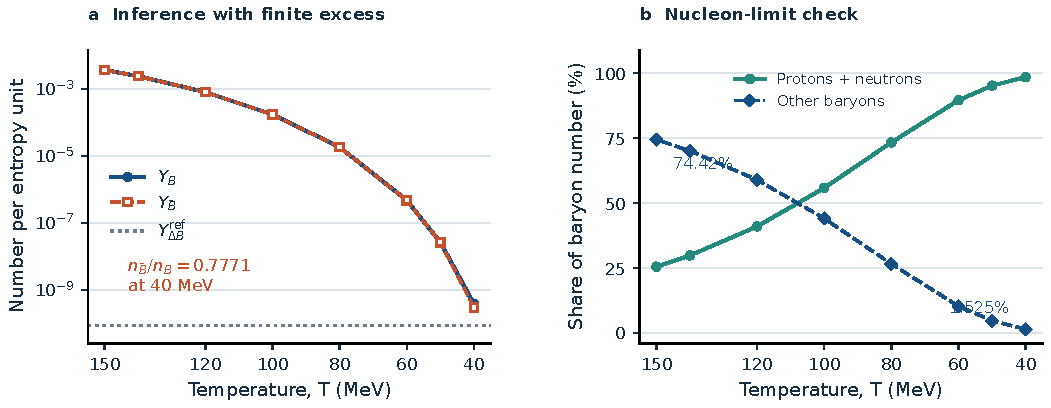
\includegraphics[width=.99\textwidth]{figures/fig05_inverse_en.pdf}
\caption{Our results addressing the retrospective objective. (a) Baryon and antibaryon yields inferred with PDG2025 and the published net excess as an input constraint. Curves nearly coincide at high temperature; their difference becomes a larger share of the total during cooling. The gray line is the conserved external constraint. (b) Shares of protons plus neutrons and of other baryons in the symmetric control. These shares were calculated here; the literature comparison uses the nucleon approximation of Satarov et al. (2013). Points are equilibrium states at specified temperatures rather than a measured kinetic trajectory.}
\label{fig:inverse}
\end{figure*}

\subsection{Quantities at alternative starting temperatures}
The 156.5-MeV transition reference corresponded to $1.8161\times10^{12}$ K. Under the same inverse conditions, PDG2025 yielded approximately $2.6575\times10^{37}$ baryons and the same rounded antibaryon density per cm$^3$. The excess was $4.8753\times10^{29}$ cm$^{-3}$, with $\mu_B/T=9.1749\times10^{-9}$. The total, $5.3150\times10^{37}$ cm$^{-3}$, exceeded the 150-MeV value by 54.31\%. Yield increased by 26.95\% to $9.4772\times10^{-3}$, distinguishing population and normalization changes. Table~\ref{tab:initialT} provides the sensitivity points. The 156.5-MeV result is our HRG evaluation at a published reference temperature, without turning it into a measured annihilation onset.

\begin{table*}[t]\centering\small
\caption{Our starting-temperature sensitivity using PDG2025 and the same net constraint. The transition reference is $156.5\pm1.5$ MeV (HotQCD, 2019); 150 MeV remains the main-grid start. The near-transition interval is neither a complete HRG uncertainty nor a measured annihilation onset.}\label{tab:initialT}
\setlength{\tabcolsep}{11pt}\renewcommand{\arraystretch}{1.14}
\begin{tabular}{rrrrr}\toprule
$T$ (MeV) & $n_B$ (${\rm cm^{-3}}$) & $n_{\bar B}$ (${\rm cm^{-3}}$) & $\Delta n_B$ (${\rm cm^{-3}}$) & $Y_\Sigma$ \\ \midrule
150 & $1.722\times10^{37}$ & $1.722\times10^{37}$ & $4.011\times10^{29}$ & 0.007465 \\
155 & $2.410\times10^{37}$ & $2.410\times10^{37}$ & $4.660\times10^{29}$ & 0.008991 \\
156.5 & $2.657\times10^{37}$ & $2.657\times10^{37}$ & $4.875\times10^{29}$ & 0.009477 \\
158 & $2.926\times10^{37}$ & $2.926\times10^{37}$ & $5.100\times10^{29}$ & 0.009976 \\
\bottomrule\end{tabular}\end{table*}


\subsection{Information recoverable from the present abundance}
The map in Eq.~\eqref{eq:rank} had rank one for two unknown components and null direction $(1,1)$. Four examples with totals of 0.1, 1, 10, and 100 times the initial total algebraically preserved $Y_B-Y_{\bar B}=8.6932\times10^{-11}$, equivalent to the same input $\eta=6.12\times10^{-10}$. The present excess alone therefore did not identify a unique initial pair population. Equilibrium at a specified temperature provided the additional information used in the reconstruction above.

\subsection{Quantitative comparison with the published nucleon limit}
Our evaluation of Eq.~\eqref{eq:nucleonMB} gave $n_p+n_n=4.4080\times10^{36}$ cm$^{-3}$ at 150 MeV in the Maxwell-Boltzmann approximation. The Fermi-Dirac sum was $4.4054\times10^{36}$ cm$^{-3}$, a relative difference of 0.05916\%. Nucleons supplied 25.5799\% of symmetric HRG baryon density; other baryons supplied 74.4201\%. At 40 MeV the nucleon share reached 98.4745\% (Table~\ref{tab:nucleoncontrast}). These numbers are our calculations using the stated approximation and catalog, rather than measured populations or values tabulated by the compared authors.

\begin{table*}[t]\centering\small
\caption{Calculated comparison with the nucleon limit of Satarov et al. (2013), generalized to distinct $p$ and $n$ masses. All numerical columns are our results at $\mu_B=0$. $\delta_{\rm MB}$ is $100(n_N^{\rm MB}/n_N^{\rm FD}-1)$; other-baryon share uses the full Fermi-Dirac HRG total.}\label{tab:nucleoncontrast}
\setlength{\tabcolsep}{8pt}\renewcommand{\arraystretch}{1.14}
\begin{tabular}{rrrrr}\toprule
$T$ (MeV) & $n_N^{\rm MB}$ (${\rm cm^{-3}}$) & $n_B^{\rm HRG}$ (${\rm cm^{-3}}$) & Other baryons (\%) & $\delta_{\rm MB}$ (\%) \\ \midrule
150 & $4.408\times10^{36}$ & $1.722\times10^{37}$ & 74.4201 & 0.05916 \\
140 & $2.498\times10^{36}$ & $8.354\times10^{36}$ & 70.1063 & 0.03814 \\
120 & $6.261\times10^{35}$ & $1.525\times10^{36}$ & 58.9552 & 0.01268 \\
100 & $9.612\times10^{34}$ & $1.720\times10^{35}$ & 44.1293 & 0.002696 \\
80 & $6.342\times10^{33}$ & $8.643\times10^{33}$ & 26.6153 & $2.623\times10^{-4}$ \\
60 & $7.938\times10^{31}$ & $8.859\times10^{31}$ & 10.3973 & $5.341\times10^{-6}$ \\
50 & $2.591\times10^{30}$ & $2.722\times10^{30}$ & 4.7824 & $2.357\times10^{-7}$ \\
40 & $1.664\times10^{28}$ & $1.690\times10^{28}$ & 1.5255 & $2.176\times10^{-9}$ \\
\bottomrule\end{tabular}\end{table*}


\subsection{Symmetric control of the initial inventory}
To check the effect of imposed symmetry, the calculation was repeated at $\mu_B=0$. The PDG2025 inventory supplied 443 active particle species: 146 baryonic, 146 antibaryonic, and 151 mesonic. These counts described particle types; populations were calculated using Eq.~\eqref{eq:number}. At $T_i=150$ MeV, our calculation gave
\begin{align}
n_B^{\rm eq}&=1.7222003\times10^{37}\ {\rm cm^{-3}},\\
n_{\bar B}^{\rm eq}&=1.7222003\times10^{37}\ {\rm cm^{-3}},\\
n_\Sigma^{\rm eq}&=3.4444006\times10^{37}\ {\rm cm^{-3}}.
\label{eq:initialpopulation}
\end{align}
For each physical cm$^3$ of plasma at this temperature, the reconstructed mean number was $1.7222\times10^{37}$ baryons and the same number of antibaryons. Symmetric bookkeeping corresponded to $1.7222\times10^{37}$ potential pairs per cm$^3$. Meson and photon densities were $2.4649\times10^{38}$ and $1.0700\times10^{38}$ cm$^{-3}$, respectively.

For nucleonic particle species we obtained $n_p=n_{\bar p}=2.2103\times10^{36}$ and $n_n=n_{\bar n}=2.1951\times10^{36}$ cm$^{-3}$. Protons and neutrons jointly supplied 25.58\% of all baryons in the inventory at 150 MeV. These were primary equilibrium populations before resonance-decay feed-down. The identity $n_B=n_{\bar B}$ gave zero net excess in the symmetric control.

\subsection{Symmetric-control abundance sequence during cooling}
Table~\ref{tab:populations} lists the reconstruction at all eight temperatures. At 40 MeV we obtained $n_B=n_{\bar B}=1.6896\times10^{28}$ cm$^{-3}$ and $n_\Sigma=3.3791\times10^{28}$ cm$^{-3}$. Total yield decreased from $Y_\Sigma^{\rm eq}=7.4653\times10^{-3}$ to $6.8756\times10^{-10}$, a reduction of 7.0357 orders of magnitude (Fig.~\ref{fig:populations}). Physical number per cm$^3$ and yield per entropy unit were retained as distinct quantities.

\begin{table*}[t]\centering\small
\caption{Equilibrium number densities reconstructed with PDG2025 at zero chemical potentials. The second column gives the density of each side; the total includes both. $Y_\Sigma=n_\Sigma/s_{\rm tot}$ separates thermal suppression from dilution. $\mathcal Q=Y_\Sigma/Y_{\Delta B}^{\rm ref}$ uses the cosmic excess as an external input. These are calculated instantaneous populations, without counting regeneration or annihilation events.}\label{tab:populations}
\setlength{\tabcolsep}{12pt}\renewcommand{\arraystretch}{1.14}
\begin{tabular}{rrrrr}\toprule
$T$ (MeV) & $n_B=n_{\bar B}$ (${\rm cm^{-3}}$) & $n_\Sigma$ (${\rm cm^{-3}}$) & $Y_\Sigma$ & $\mathcal Q$ \\ \midrule
150 & $1.722\times10^{37}$ & $3.444\times10^{37}$ & 0.007465 & $8.587\times10^{7}$ \\
140 & $8.354\times10^{36}$ & $1.671\times10^{37}$ & 0.004887 & $5.622\times10^{7}$ \\
120 & $1.525\times10^{36}$ & $3.051\times10^{36}$ & 0.001634 & $1.880\times10^{7}$ \\
100 & $1.720\times10^{35}$ & $3.441\times10^{35}$ & $3.506\times10^{-4}$ & $4.033\times10^{6}$ \\
80 & $8.643\times10^{33}$ & $1.729\times10^{34}$ & $3.687\times10^{-5}$ & $4.241\times10^{5}$ \\
60 & $8.859\times10^{31}$ & $1.772\times10^{32}$ & $9.595\times10^{-7}$ & $1.104\times10^{4}$ \\
50 & $2.722\times10^{30}$ & $5.443\times10^{30}$ & $5.331\times10^{-8}$ & 613.2 \\
40 & $1.690\times10^{28}$ & $3.379\times10^{28}$ & $6.876\times10^{-10}$ & 7.909 \\
\bottomrule\end{tabular}\end{table*}

\begin{figure*}[t]
\centering
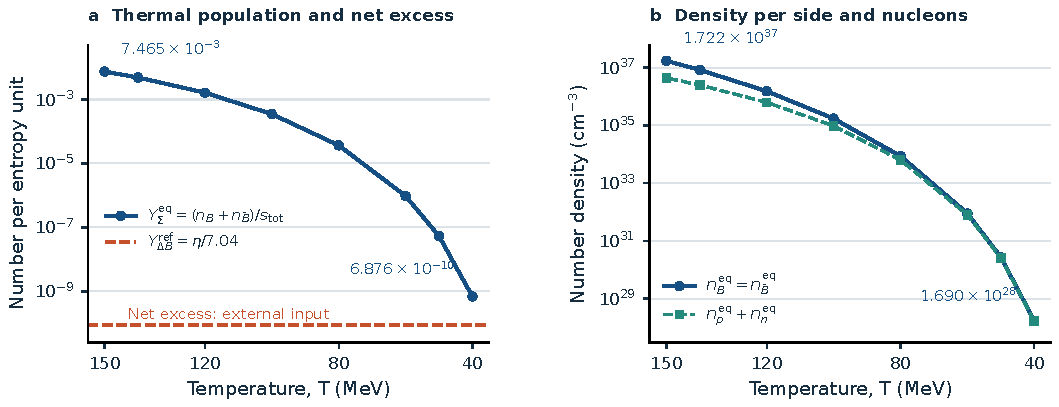
\includegraphics[width=.99\textwidth]{figures/fig04_populations_en.pdf}
\caption{Our reconstruction of number populations using PDG2025. (a) Total thermal yield $Y_\Sigma^{\rm eq}$ and reference net excess $Y_{\Delta B}^{\rm ref}=8.6932\times10^{-11}$. The net-excess line uses an external cosmic normalization; the blue curve was calculated from the HRG inventory. (b) Density of each symmetric side and the proton-plus-neutron contribution. Each antiparticle curve coincides with its particle counterpart in the symmetric control. Axes follow cooling and segments guide the eye. These are instantaneous equilibrium populations, without counting cumulative annihilation or regeneration events.}
\label{fig:populations}
\end{figure*}


\subsection{Comparison at fixed temperature}
All three larger lists produced fractions that decreased throughout the temperature grid during cooling (Table~\ref{tab:comparison}; Figure~\ref{fig:comparison}). PDG2025 yielded
\begin{align}
\fB(150\ {\rm MeV})&=0.08454533,\\
\fB(40\ {\rm MeV})&=1.7970078\times10^{-8}.
\end{align}
The first value is 8.4545\%, whereas the second is $1.7970\times10^{-6}\%$.

\begin{table*}[t]\centering\footnotesize
\caption{Comparison at fixed temperature of the baryon-antibaryon entropy fraction. The four $f$ columns are dimensionless fractions; the last two are percentages. The reduced reference was transcribed from the prior manuscript; the PDG columns were calculated in this audit with the same light plasma. The descriptive ratio was evaluated before rounding the PDG result.}\label{tab:comparison}
\setlength{\tabcolsep}{9pt}\renewcommand{\arraystretch}{1.14}
\begin{tabular}{rrrrrrr}\toprule
$T$ (MeV) & $f_{\mathrm{prior}}$ & $f_{\mathrm{PDG2014}}$ & $f_{\mathrm{PDG2020}}$ & $f_{\mathrm{PDG2025}}$ & $100R$ & $100d$ \\ \midrule
150 & 0.06208 & 0.08351 & 0.08459 & 0.08455 & 73.43 & 26.57 \\
140 & 0.04328 & 0.05633 & 0.05695 & 0.05693 & 76.02 & 23.98 \\
120 & 0.01686 & 0.02018 & 0.02032 & 0.02032 & 82.97 & 17.03 \\
100 & 0.004305 & 0.004734 & 0.00475 & 0.00475 & 90.64 & 9.36 \\
80 & $5.464\times10^{-4}$ & $5.655\times10^{-4}$ & $5.661\times10^{-4}$ & $5.661\times10^{-4}$ & 96.52 & 3.48 \\
60 & $1.782\times10^{-5}$ & $1.795\times10^{-5}$ & $1.795\times10^{-5}$ & $1.795\times10^{-5}$ & 99.26 & 0.74 \\
50 & $1.148\times10^{-6}$ & $1.152\times10^{-6}$ & $1.152\times10^{-6}$ & $1.152\times10^{-6}$ & 99.67 & 0.33 \\
40 & $1.795\times10^{-8}$ & $1.797\times10^{-8}$ & $1.797\times10^{-8}$ & $1.797\times10^{-8}$ & 99.89 & 0.11 \\
\bottomrule\end{tabular}\end{table*}

\begin{figure*}[t]
\centering
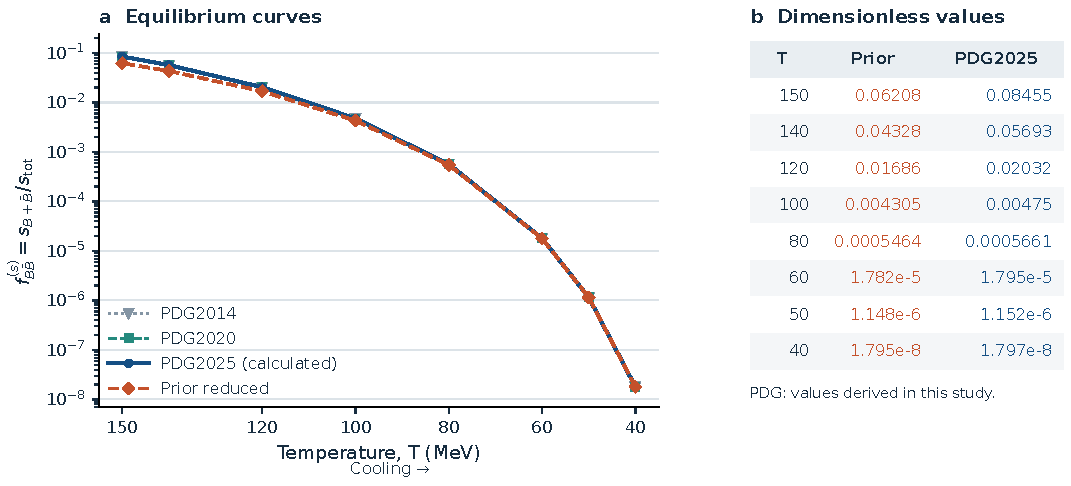
\includegraphics[width=.99\textwidth]{figures/fig01_comparison_en.pdf}
\caption{Baryon-antibaryon entropy fraction at vanishing chemical potentials. (a) Semilogarithmic comparison of the reduced reference with three independent calculations using Thermal-FIST lists based on PDG2014, PDG2020, and PDG2025. The horizontal axis follows cooling from left to right. (b) Dimensionless values of the reference and the PDG2025 calculation at all eight temperatures. Every PDG curve is a result derived in this calculation, with zero resonance widths and a common light sector in the denominator, rather than an external measurement. Segments connect calculated points as visual guides.}
\label{fig:comparison}
\end{figure*}

At 150 MeV, the prior reference of 6.208\% lay 2.2465 percentage points below the PDG2025 calculation. The ratio $R$ was 0.73428 and the relative deficit was 26.57\%. During cooling, $100R$ increased to 90.64\% at 100 MeV, 99.26\% at 60 MeV, and 99.89\% at 40 MeV (Figure~\ref{fig:convergence}). The maximum spread across lists on the grid occurred at 150 MeV: 0.10775 percentage points. Their percentages there were 8.3509, 8.4586, and 8.4545\% for PDG2014, PDG2020, and PDG2025, respectively.

\begin{figure*}[t]
\centering
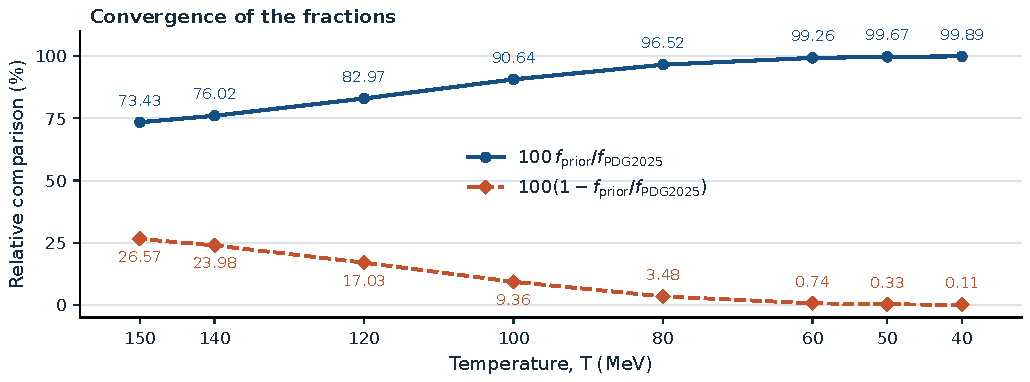
\includegraphics[width=.99\textwidth]{figures/fig02_convergence_en.pdf}
\caption{Relative contrast between the prior reduced reference and the PDG2025 calculation. Blue points show $100R=100f_{\rm prior}/f_{25}$; orange points show its complement, $100d=100(1-R)$. Labels report percentages calculated before rounding $f_{25}$, using the four significant digits available for the prior reference. These quantities measure numerical agreement between equilibrium fractions; they are neither validation probabilities nor percentages of annihilated pairs.}
\label{fig:convergence}
\end{figure*}

\subsection{Shape of the series}
Correlation between the logarithms of the eight fractions was $r_{\log}=0.9999233$, with $\mathrm{RMSE}_{\log}=0.0714338$. The endpoint ratio was $2.89143\times10^{-7}$ for the reduced reference and $2.12550\times10^{-7}$ for PDG2025. Corresponding decreases were 6.539 and 6.673 orders of magnitude. Spearman's rank correlation was $\rho_S=1$, consistent with the common monotonic ordering. These metrics summarized series shape and amplitude differences on the selected grid.

\subsection{Densities and denominator effect}
PDG2025 at 150 MeV gave the following densities:
\begin{align}
\sB&=2.9972147\times10^{-3}\ {\rm GeV^3},\\
s_{\rm mes}&=1.1626411\times10^{-2}\ {\rm GeV^3},\\
\shad&=1.4623626\times10^{-2}\ {\rm GeV^3},\\
\sL&=2.0827352\times10^{-2}\ {\rm GeV^3},\\
\stot&=3.5450978\times10^{-2}\ {\rm GeV^3}.
\end{align}
The partition of $\stot$ was 8.4545\% baryons and antibaryons, 32.7957\% mesons, and 58.7497\% light sector. Using $\shad$ alone as the denominator gave 20.4957\% for the same numerator (Figure~\ref{fig:denominator}).

\begin{figure*}[t]
\centering
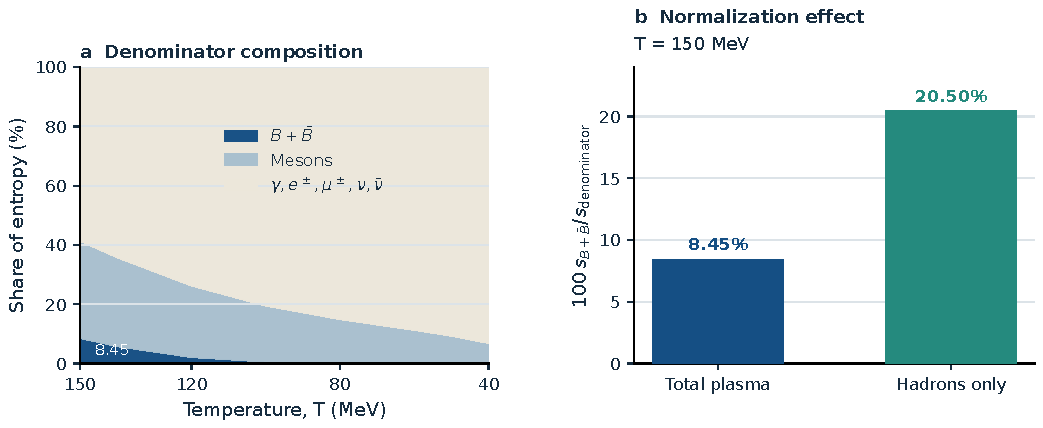
\includegraphics[width=.99\textwidth]{figures/fig03_denominator_en.pdf}
\caption{Effect of the total-entropy definition in the PDG2025 calculation. (a) Shares of baryons and antibaryons, mesons, and the light sector in $\stot$ at all eight temperatures; areas between points are visual guides. (b) The same numerator $\sB$ at 150 MeV represents 8.45\% of the entropy of the selected plasma and 20.50\% of exclusively hadronic entropy. The change reflects normalization rather than a different baryonic population. The figure describes instantaneous equilibrium composition, without identifying the individual fate of annihilation products.}
\label{fig:denominator}
\end{figure*}

\subsection{Relic scale and connection with H and He}
Normalization to the external excess $\YB^{\rm ref}=8.6932\times10^{-11}$ gave $\mathcal Q(150)=8.5875\times10^7$ and $\mathcal Q(40)=7.9092$. Per reference unit of net baryon number, the initial symmetric population represented $4.2937\times10^7$ baryons and the same number of antibaryons. This comparison used a common comoving normalization. At 40 MeV the symmetric equilibrium total remained 7.91 times that excess; the grid endpoint was not a calculated final relic.

Observational inputs and Eqs.~\eqref{eq:today} and \eqref{eq:hydrogen} gave Table~\ref{tab:present}. The inferred mean baryon density was $(2.514\pm0.017)\times10^{-7}$ cm$^{-3}$, or $0.2514\pm0.0017$ baryon-number units per m$^3$. Within input rounding, this agreed with the reference $(2.515\pm0.017)\times10^{-7}$ cm$^{-3}$ compiled by \citet{Groom2025}. Both conversions shared the CMB normalization.

\begin{table}[t]
\centering\small
\caption{Conversions calculated from published cosmological inputs. Uncertainties use first-order input propagation, excluding HRG physical uncertainties. H, He, and D denote a primordial-composition equivalent at today's mean density, rather than a census of present neutral atoms.}
\label{tab:present}
\setlength{\tabcolsep}{3pt}\renewcommand{\arraystretch}{1.18}
\begin{tabular}{lr}\toprule
Quantity & Density (${\rm cm^{-3}}$)\\\midrule
CMB photons & $410.73\pm0.27$\\
Net baryon number & $(2.514\pm0.017)\times10^{-7}$\\
H nuclei & $(1.898\pm0.015)\times10^{-7}$\\
$^4$He nuclei & $(1.540\pm0.021)\times10^{-8}$\\
D nuclei & $(4.760\pm0.066)\times10^{-12}$\\
\bottomrule\end{tabular}
\end{table}

The retrospective sequence was: present abundance, conservation constraint on net yield, HRG inventory properties, specified temperature, and solution for early populations. H/He/D conversions described the cosmological reference used, rather than independent HRG predictions.

\subsection{Numerical and chemical checks}
Number-density quadrature and series differed by less than $5\times10^{-16}$ at recorded precision. We exported 3544 records for 443 particle species at eight temperatures.

Doubling the series length did not change the fractions at the recorded arithmetic precision. Independent integrals met the $10^{-8}$ criterion for all tested species and temperatures. The massless-electron approximation overestimated electron entropy by relative amounts of $1.26\times10^{-6}$ at 150 MeV and $1.77\times10^{-5}$ at 40 MeV.

The inverse solution closed the net constraint with a maximum relative error of $2.23\times10^{-15}$ across the three lists. Changes on doubling the number of terms were below $4.5\times10^{-16}$. Independent nucleon-excess integrals agreed with the sums within a relative $3.83\times10^{-13}$. At 40 MeV, the finite excess increased total baryon-plus-antibaryon density by 0.7961\% relative to the symmetric control. Validation files distinguished this reconstruction from zero-potential checks.

\section{Discussion}
\subsection{Answer to the reconstruction objective}
The results support a conditional quantitative answer: particle-species properties and observed net abundance, together with an explicit temperature and equilibrium model, reconstructed baryons and antibaryons separately. The inverse constraint incorporated the published excess into the calculation instead of only comparing it afterwards with a symmetric population. At 150 MeV, approximately $1.7222\times10^{37}$ particles per cm$^3$ were inferred on each side, with a small difference of $4.0110\times10^{29}$ cm$^{-3}$. At 40 MeV, the same net constraint distinguished $1.9166\times10^{28}$ baryons from $1.4894\times10^{28}$ antibaryons per cm$^3$.

The rank test clarified what information comes from the present. Net abundance fixes a difference; adding equal numbers of particles and antiparticles leaves it unchanged. Masses and present abundance without additional thermal conditions therefore do not determine how many pairs existed. HRG equilibrium at a specified temperature supplies this extra relation. The resulting reconstruction is an inference under testable assumptions, rather than unique recovery of a lost historical record.

The 150-MeV upper endpoint is the chosen initial point in the hadronic regime considered. A universal date at which every particle species began annihilating was not identified. \emph{Reconstructed} quantities is accurate; a total number of \emph{regenerated} events requires time-dependent inverse reactions.

The total-density spread across the three lists at 150 MeV was 1.185\% of the PDG2025 value. Starting-temperature sensitivity was larger: changing from 150 to 156.5 MeV increased reconstructed physical density by 54.31\% and yield by 26.95\%. Each quantity therefore requires an explicit temperature. The reference of \citet{Bazavov2019} supplies a physical scale for hadron formation; a specific kinetic onset still requires reaction rates and expansion. Near the transition, checking HRG against the QCD equation of state is necessary before assigning physical precision to the count.

\subsection{Agreement with published knowledge}
Our comparison with the nucleon limit of \citet{Satarov2013} showed a difference of only 0.05916\% between Maxwell-Boltzmann and Fermi-Dirac proton-plus-neutron densities at 150 MeV. The difference between nucleons alone and the full inventory was much larger: other baryons supplied 74.42\% at that temperature, 44.13\% at 100 MeV, and 1.525\% at 40 MeV. These calculated shares agree with the importance of heavy resonances at high temperature described by those authors. The comparison separates inventory effects from the distribution approximation.

Their kinetic evolution and interaction corrections were not reproduced. Nor does this provide direct observational verification of early densities. The literature supplied an approximation and a reference behavior; our code evaluated quantities under stated common assumptions. At 40 MeV, the inferred total remained 7.97 times the net excess, so the lower endpoint was not a final relic abundance.

Entropy curves retained the reduced reference's decrease, with their largest discrepancy at 150 MeV. In the nonrelativistic limit $x_i=m_i/T\gg1$,
\begin{equation}
\frac{s_i}{T^3}\simeq
\frac{g_i}{(2\pi)^{3/2}}x_i^{3/2}
\left(x_i+\frac{5}{2}\right)e^{-x_i}.
\label{eq:asymptotic}
\end{equation}
This suppression explains why higher masses lose contribution during cooling. The reduced reference lacks a complete inventory and original code, retaining the scope of a transcription. High correlation describes shared series shape rather than physical accuracy or validation of a matter-origin hypothesis.

\subsection{Own contribution and scope of novelty}
The verifiable contribution was explicit numerical reconstruction using frozen inventories, inverse linkage to present excess, separate particle and antiparticle accounting, and reproducible checks. New tables and shares are results of our calculations. Annihilation mechanisms, thermal distributions, and HRG methods are established in the literature \citep{Vovchenko2019,Satarov2013}. The information limit of a net difference is a mathematical property of the problem.

This study did not establish a new physical mechanism, particle species, or independent prediction of cosmic asymmetry or present hydrogen. The comparison evaluates quantitative agreement and differences but does not establish priority or novelty against the entire literature. Such a claim requires a dedicated prior-work review and a result distinguishable from earlier predictions under equivalent conditions.

\subsection{Sequence connecting current abundances}
Table~\ref{tab:external} declares each reference's role. The 2025 BBN review includes deuterium measurements such as \citet{Cooke2018} and recommends the average used here. First, $\eta$ fixed net yield; second, HRG properties and temperature reconstructed early populations; third, $\eta$ and CMB temperature gave today's mean baryon density; finally, $Y_p$ and D/H supplied an equivalent primordial composition in H, He, and D.

The equivalent H density, $(1.898\pm0.015)\times10^{-7}$ cm$^{-3}$, depends on these additional inputs. Its calculation is not an independent HRG nuclear prediction. Agreement of baryon density with the published table checks a conversion sharing the CMB input. Nuclear abundances require evolution through BBN and a reaction network \citep{Fields2025}; a census of present neutral hydrogen also requires stellar processing and ionization.

\begin{table*}[t]
\centering\small
\caption{Published references and their roles in reconstruction. Uncertainties are those of the sources, with declared rounding for $T_{\gamma0}$; FIRAS limits are at 95\% confidence. Calculation inputs are distinguished from comparison channels not fitted in this study.}
\label{tab:external}
\setlength{\tabcolsep}{5pt}\renewcommand{\arraystretch}{1.15}
\begin{tabular}{>{\raggedright\arraybackslash}p{.18\textwidth}>{\raggedright\arraybackslash}p{.23\textwidth}>{\raggedright\arraybackslash}p{.22\textwidth}>{\raggedright\arraybackslash}p{.26\textwidth}}\toprule
Observable & Published value & Source & Role in reconstruction\\\midrule
CMB $\eta_{10}$ & $6.12\pm0.04$ & \citet{Fields2025} & Net constraint on inverse inference.\\
Current CMB temperature & $2.7255\pm0.0006$ K & \citet{Fixsen2009}, rounded & Photon density and current normalization.\\
$^4$He baryon fraction & $Y_p=0.245\pm0.003$ & \citet{Fields2025} & Approximate H and He conversion.\\
Primordial deuterium & $(2.508\pm0.029)\times10^{-5}$ & \citet{Fields2025} & Approximate D conversion.\\
Current baryon density & $(2.515\pm0.017)\times10^{-7}$ cm$^{-3}$ & \citet{Groom2025} & Conversion check; shared CMB input.\\
Density $\Omega_bh^2$ & $0.02237\pm0.00015$ & \citet{Planck2020} & External reference; no cosmological model fitted.\\
Spectral distortions & $|y|<1.5\times10^{-5}$\newline $|\mu|<9\times10^{-5}$ & \citet{Fixsen1996} & Relevant constraint on future late energy injection.\\
\bottomrule\end{tabular}
\end{table*}

The factor 7.04 uses the standard entropy-per-photon approximation after $e^+e^-$ annihilation. Precise neutrino-decoupling calculations include corrections \citep{Froustey2020}; this factor was not treated as a measured parameter with uncertainty here.

\subsection{Equilibrium populations and annihilation history}
In adiabatic expansion, $S_{\rm com}=\stot a^3$ is approximately conserved. A schematic evolution with annihilation and inverse production is \citep{Satarov2013}
\begin{align}
\dot n_B+3Hn_B&=-\mathcal C,\\
\dot n_{\bar B}+3Hn_{\bar B}&=-\mathcal C,\\
\mathcal C&=\langle\sigma v\rangle
\bigl(n_Bn_{\bar B}-n_B^{\rm eq}n_{\bar B}^{\rm eq}\bigr).
\end{align}
Subtracting the equations gives $\dot{\Delta n}_B+3H\Delta n_B=0$. This justifies using conserved excess as a retrospective link under the adopted assumptions. Cumulative events require separate time-and-volume integration of production and loss. A sequence of equilibrium states does not supply those totals.

\subsection{Reconstruction limitations}
Nominal masses, zero widths, an ideal gas, and common temperature were used without lattice fits or mass, spin, and interaction uncertainties. The net constraint did not simultaneously solve charge and strangeness neutrality. Checks established numerical precision rather than physical accuracy of these assumptions. Proximity of 150 MeV to the transition requires evaluating model corrections before assigning physical uncertainties \citep{Bazavov2012}.

Cosmological uncertainties were propagated only to current conversions; inverse populations used central inputs. Catalog spread is sensitivity to correlated inventories. The study did not identify kinetic onset, integrate reaction rates, or generate primordial asymmetry \citep{Sakharov1967}. Within this scope it establishes conditional early quantities and an explicit comparison with available knowledge.

\section{Conclusions}
Rest masses and other HRG properties, observed net excess, and specified equilibrium temperatures reconstructed separate baryon and antibaryon populations. At 150 MeV, approximately $1.7222\times10^{37}$ cm$^{-3}$ were inferred per side, with excess $4.0110\times10^{29}$ cm$^{-3}$. At 40 MeV, $n_B=1.9166\times10^{28}$ and $n_{\bar B}=1.4894\times10^{28}$ cm$^{-3}$. Total yield fell 7.0323 orders of magnitude.

Present abundance alone did not determine initial pairs: the rank-one net map preserved equal additions to both components. Equilibrium at fixed temperature supplied additional information. The published nucleon-limit comparison gave other-baryon shares of 74.42\% at 150 MeV and 1.525\% at 40 MeV.

The $T_c=156.5\pm1.5$ MeV reference motivated an initial-temperature check. At its central value, the HRG gave approximately $2.6575\times10^{37}$ cm$^{-3}$ per side, with total density 54.31\% above the 150-MeV result. This quantified sensitivity without identifying a measured annihilation onset.

Current references, $n_{b0}=(2.514\pm0.017)\times10^{-7}$ cm$^{-3}$ and primordial H equivalent $(1.898\pm0.015)\times10^{-7}$ cm$^{-3}$, were conversions of observational inputs. The conditional reconstruction did not establish a new physical discovery or unique history. Cumulative events and final nuclear abundances require reaction rates and cosmological evolution.

\section*{Data and code availability}
The supplement contains frozen catalogs and hashes, entropy and number densities, 3544 PDG2025 control records, 24 inverse states, 12 initial-temperature evaluations, the nucleon comparison, rank test, cosmological conversions, numerical checks, five figures per language, and manuscript sources. The included independent Python implementation used Thermal-FIST data under their original license.

\section*{Preparation assistance}
Artificial-intelligence assistance supported writing, code, figures, and layout. Reported sums, integrals, and inverse solutions were executed and retained. Scientific evaluation and publication remain the author's responsibility.



\onecolumn
\begin{multicols}{2}
\begin{thebibliography}{99}\small
\setlength{\itemsep}{2pt}
\bibitem[Bazavov et al.(2012)]{Bazavov2012}
Bazavov, A., Bhattacharya, T., DeTar, C. E., Ding, H.-T., Gottlieb, S., Gupta, R., Hegde, P., Heller, U. M., Karsch, F., Laermann, E., Levkova, L., Mukherjee, S., Petreczky, P., Schmidt, C., Soltz, R. A., Soeldner, W., Sugar, R., \& Vranas, P. M. (2012).
Fluctuations and correlations of net baryon number, electric charge, and strangeness: A comparison of lattice QCD results with the hadron resonance gas model.
\emph{Physical Review D, 86}, 034509. \doi{10.1103/PhysRevD.86.034509}.

\bibitem[Bazavov et al.(2019)]{Bazavov2019}
Bazavov, A., Ding, H.-T., Hegde, P., Kaczmarek, O., Karsch, F., Karthik, N., Laermann, E., Lahiri, A., Larsen, R., Li, S.-T., Mukherjee, S., Ohno, H., Petreczky, P., Sandmeyer, H., Schmidt, C., Sharma, S., \& Steinbrecher, P. (HotQCD Collaboration). (2019).
Chiral crossover in QCD at zero and non-zero chemical potentials.
\emph{Physics Letters B, 795}, 15--21. \doi{10.1016/j.physletb.2019.05.013}.

\bibitem[Cooke et al.(2018)]{Cooke2018}
Cooke, R. J., Pettini, M., \& Steidel, C. C. (2018).
One percent determination of the primordial deuterium abundance.
\emph{The Astrophysical Journal, 855}(2), 102.
\doi{10.3847/1538-4357/aaab53}.

\bibitem[Fields et al.(2025)]{Fields2025}
Fields, B. D., Molaro, P., \& Sarkar, S. (2025).
Big Bang nucleosynthesis. In \emph{Review of Particle Physics: 2025 update}.
\href{https://pdg.lbl.gov/2025/reviews/rpp2025-rev-bbang-nucleosynthesis.pdf}{PDG review}.

\bibitem[Fixsen(2009)]{Fixsen2009}
Fixsen, D. J. (2009).
The temperature of the cosmic microwave background.
\emph{The Astrophysical Journal, 707}(2), 916--920.
\doi{10.1088/0004-637X/707/2/916}.

\bibitem[Fixsen et al.(1996)]{Fixsen1996}
Fixsen, D. J., Cheng, E. S., Gales, J. M., Mather, J. C., Shafer, R. A., \& Wright, E. L. (1996).
The cosmic microwave background spectrum from the full COBE/FIRAS data set.
\emph{The Astrophysical Journal, 473}, 576--587.
\doi{10.1086/178173}.

\bibitem[Froustey et al.(2020)]{Froustey2020}
Froustey, J., Pitrou, C., \& Volpe, M. C. (2020).
Neutrino decoupling including flavour oscillations and primordial nucleosynthesis.
\emph{Journal of Cosmology and Astroparticle Physics, 2020}(12), 015.
\doi{10.1088/1475-7516/2020/12/015}.

\bibitem[García(2026)]{Garcia2026}
García, A. G. (2026).
\emph{From matter-antimatter annihilation to the baryonic relic: Entropy transfer across the hadronic epoch}
[Unpublished working manuscript, v0.9]. Independent Researcher, Mexico.

\bibitem[Groom and Scott(2025)]{Groom2025}
Groom, D. E., \& Scott, D. (2025).
Astrophysical constants and parameters. In \emph{Review of Particle Physics: 2025 update}, Table 2.1.
\href{https://pdg.lbl.gov/2025/reviews/rpp2025-rev-astrophysical-constants.pdf}{PDG constants table}.

\bibitem[Particle Data Group(2025)]{PDG2025}
Particle Data Group. (2025).
Muon properties. In \emph{Review of Particle Physics: 2025 update}.
\href{https://pdg.lbl.gov/2025/listings/rpp2025-list-muon.pdf}{PDG muon listing}.

\bibitem[Planck Collaboration(2020)]{Planck2020}
Planck Collaboration. (2020).
Planck 2018 results. VI. Cosmological parameters.
\emph{Astronomy \& Astrophysics, 641}, A6.
\doi{10.1051/0004-6361/201833910}.

\bibitem[Robinson and Zyla(2025)]{Robinson2025}
Robinson, D., \& Zyla, P. A. (2025).
Physical constants. In \emph{Review of Particle Physics: 2025 update}, Table 1.1.
\href{https://pdg.lbl.gov/2025/reviews/rpp2025-rev-phys-constants.pdf}{PDG physical constants}.

\bibitem[Sakharov(1967)]{Sakharov1967}
Sakharov, A. D. (1967).
Violation of CP invariance, C asymmetry, and baryon asymmetry of the universe.
\emph{JETP Letters, 5}, 24--27.

\bibitem[Satarov et al.(2013)]{Satarov2013}
Satarov, L. M., Mishustin, I. N., \& Greiner, W. (2013).
Evolution of antibaryon abundances in the early Universe and in heavy-ion collisions.
\emph{Physical Review C, 88}, 024908.
\doi{10.1103/PhysRevC.88.024908}.

\bibitem[Vovchenko and Stoecker(2019)]{Vovchenko2019}
Vovchenko, V., \& Stoecker, H. (2019).
Thermal-FIST: A package for heavy-ion collisions and hadronic equation of state.
\emph{Computer Physics Communications, 244}, 295--310.
\doi{10.1016/j.cpc.2019.06.024}.

\bibitem[Vovchenko and Stoecker(2026)]{TFLists2026}
Vovchenko, V., \& Stoecker, H. (2026).
\emph{Thermal-FIST: PDG2014, PDG2020, and PDG2025 light-and-strange particle lists}
[Data files, repository snapshot \texttt{4086191e9522}].
\href{https://github.com/vlvovch/Thermal-FIST/tree/4086191e952285cd572ba2bbbefb2fdc55401c9b/input/list}{GitHub repository snapshot}.

\end{thebibliography}


\end{multicols}
\end{document}

